\documentclass{article}
\usepackage{amsmath,amssymb,graphicx,subfig}

\title{SPL-10473-2011, Inference in Hidden Markov Models with Explicit State Duration Distributions - Response to Reviewers}

\begin{document}
\maketitle
We would like to thank the reviewers for their encouraging comments. Below we respond to each reviewer in turn.

\section*{Reviwer 1}

We would like to thank reviewer 1 for the detailed response. We have corrected all the typos mentioned and included the reference on speech synthesis. 

Reviewer 1 has suggested the comparison of our proposed method with Gibbs sampling and the Forward Backward algorithm. We found that we do not have sufficient space to introduce a meaningful comparison to the either.  We do here, however, show additional experiments which may help address the reviewer's concern.  We hope that the corrections we made to our prose will be sufficient to explain away many of the reviewers' concerns about the note.

The first suggested comparison is to a Gibbs sampler.  The Gibbs sampler was too casually mentioned in the original text as Gibbs sampling would require block-sampling in a model augmented with state-change-boundary auxiliary indicator variables.   We have edited the introduction to section 3 and included an additional reference to a paper that samples in this representation and reports the kind of mixing/computational problems that we previously hinted at.

The second suggestion was to use the forward-backward algorithm to perform inference. This can be achieved by artificially setting the auxiliary variable $u$ to zero, and hence accepting each transition in the sampler, but then requires $O(T^3K^2)$ total cost which is impractical for even the short toy data examples provided in the paper. To get out of this re-introduces the problem we set out to solve: how to choose a range of possible durations over which to sample. One way to do this in a manner that is guaranteed not to break, is to allow any duration up to the length of the sequence. Since this is computationally infeasable (see the caption to Figure 4), we can, instead, show the achieved expected joint-likelihood of the model and the data as we increase $d_\mathrm{max}$.  This unsurprisingly breaks exactly as we would expect it to.  This graph shows the mean likelihood of the samples after burn-in as the maximum duration increases, and shows one way that the truncated forward/backward algorithm suffers when the true durations are not in the support of the truncation windows.   We have placed the code for this experiment in the code repository and include a quick graph below. The mean likelihood of the beam sampler is shown in purple for comparison. 

MIKE: IF THERE ARE NO STATES OF DURATIONS GREATER THAN 25 IN THE DATA THEN I DONT BELIEVE THIS FIGURE.  IF $d_{max}$ IS SET LARGER THAN THE BIGGEST OBSERVED SEQUENCE THEN THESE FIGURES SHOULD OVERLAP.  I DON'T KNOW WHAT DATA THIS FIGURE CORRESPONDS TO AND WHAT DURATIONS ARE IN THE DATA.  IT MIGHT MAKE SENSE TO RUN THESE EXPERIMENTS OUT TO OVERLAP.  IT SHOULD BE POSSIBLE.  

\begin{figure}
	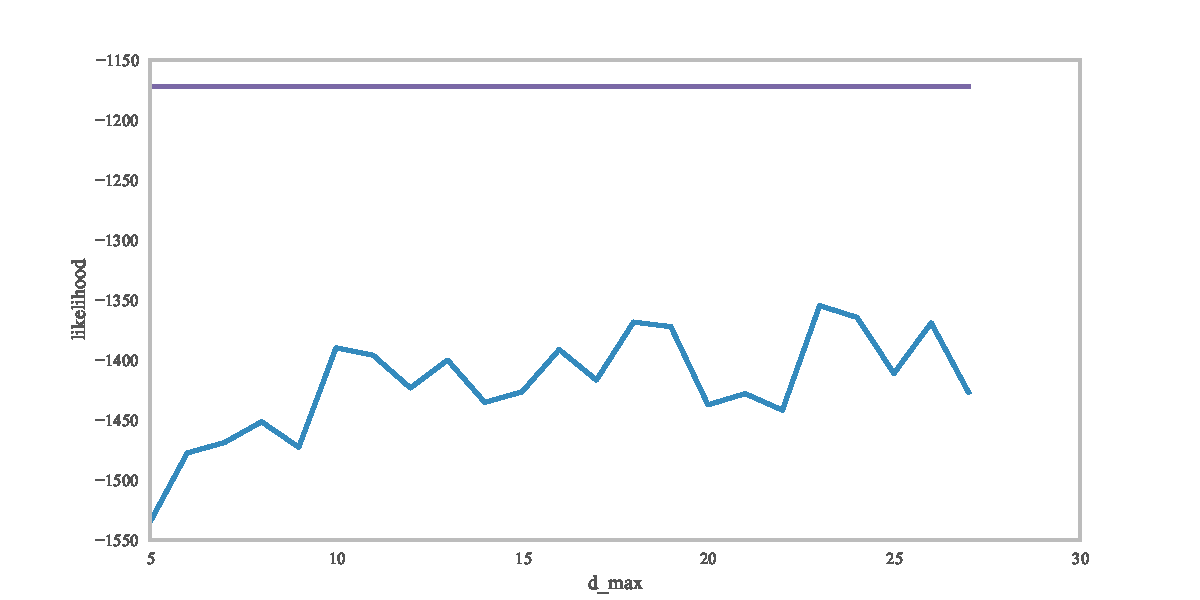
\includegraphics[width=0.8\textwidth]{../pic/likelihood_over_dmax.pdf}
	\caption{Mean likelihood over samples after burn-in as the range of possible durations increases (blue line). Shown for comparison is the mean likelihood of the beam sampler (purple line)}
\end{figure}


\section*{Reviwewr 2}

We thank the reviewer for their comments, we have addressed the typos. 

\section*{Reviewer 3}

Reviewer 3 has highlighted two omissions in the paper. The first was that we did not make clear the fact that the Explicit Duration HMM is a type of Hidden Semi Markov Model, which is now made clear in the second paragraph of the introduction, along with an additional citation to an HSMM review detailing the relationship. The second was that we did not report on the results of the transition rate parameter estimates. While we do not report any detailed results for these parameters, as they are not the focus of the paper, we have made sure to report that this estimation is done. The reader is able to reproduce our experiments using the code online for more detailed investigation if necessary. 

We were unable to include all of the references mentioned due to the space limitations of the paper, however we have made sure to include one speech-synthesis paper, also suggested by reviewer 1, by Zen et al to make sure this application area is represented in the text. 

\section*{Reviewer 4}

We thank the reviewer for their comments, and have fixed the typos. 
\end{document}